\chapter[Background]{Motivation and context}\label{ch_Background}

\begin{chapsumm}
\cstitle{This chapter at a glance}
\begin{itemize}
\item Problems with machine learning in social and political domains
\item Contrasting socio-political theories of fairness in decision systems
\item The history, application and interpretation of anti-discrimination law
\item Association paradoxes and the importance of domain knowledge
\item The different types of harm caused by biased systems
\end{itemize}
\end{chapsumm}
%
\noindent
%
Welcome and congratulations on taking this first step towards becoming a better machine learning practitioner and citizen of the world. If you've made it here chances are you've already worked with models and have some awareness of the problem of unfair machine learning algorithms. You might be a student with a foundational course in machine learning under your belt, or a Data Scientist or Machine Learning Engineer, concerned about the impact your models might have on the world. In this book we are going to learn a whole host of techniques for measuring and mitigating bias and unfairness from machine learning models. We will implement them in Python using Jupyter Notebook and analyse their behaviour. In this book I will assume you have some experience with the Python data science stack (Pandas, NumPy, SciPy, Matplotlib and scikit-learn). At the end of this book you will be able to make educated choices about which techniques and methods to use for measuring and mitigating bias in your own models. We will work with IBMs AI Fairness 360 (AIF360) library, the most comprehensive open source library  available for measuring and mitigating bias in machine learning models.

Before we embark on this journey it's important to look at the bigger picture. Bias and fairness in machine learning is a complex topic. It is not simply a matter of evaluating some formulas, implementing an algorithm, optimising a value or writing some code. These are critical components, and we'll spend much of this book on such challenges, but the problem of unfair bias in machine learning models is very much an interdisciplinary one. The choices we make in developing machine learning solutions can raise questions that are ethical, social, political, legal and philosophical in nature. Given this, we would be remiss not to start with the broader context to motivate our learning and better understand the multifaceted nature of the problem.

As we'll see in this chapter, building fair models is hard for a whole host of reasons. Fairness is not free, it requires resources. In industry where models are developed and deployed for profit, and companies compete for market share, there are strong incentives to minimise cost and decrease the time to deployment; a strategy not particularly conducive to taking a careful, considered approach. Data can be misleading - we'll see that identifying bias from static data is not just a matter of crunching numbers. Identifying causal relationships requires domain knowledge - an understanding of the data and metrics. Fairness is a rather subjective notion. Correspondingly there is no single fairness metric one can calculate to know if any given model is fair, or single solution to making a system fairer. How does one decide which metric is the right one and whose responsibility is it to decide? Context is everything and this is one of the two main purposes of this chapter - to provide context. The other is motivation. Why is it important to consider the fairness of our models? What happens if we don't? What's the harm? What does the law say and how does it ensure models are fair? These are some of the questions we'll focus on in this chapter.

We'll start with a brief recap of the different types of machine learning disciplines. We'll discuss machine learning in the context of modelling and advocate for a healthy level of scepticism towards models and their ability to `learn' and predict the future. We will discuss some theories of fairness in sociopolitical systems that can be related to model training and criteria. We will look at anti-discrimination laws in the US - discuss briefly the history and application of them, and the tensions that exist in their interpretation. We will discuss technical difficulties in identifying bias in data through illustrative examples of Simpson's paradox. Finally we will learn about the different types of harm that are caused by biased systems - many of which are difficult if not impossible to quantify. By the end of this chapter we will have a stronger more grounded sense of why fairness of machine learning systems is important.

%%%%%%%%%%%%%%%%%%%%%%%%%%%%%%%%%%%%%%%%%%%%%%%%%%%%%%%%%%%%%%%%%%%%%%%%%%%%
%%%%%%%%%%%%%%%%%%%%%%%%%%%%%%%%%%%%%%%%%%%%%%%%%%%%%%%%%%%%%%%%%%%%%%%%%%%%
%%%%%%%%%%%%%%%%%%%%%%%%%%%%%%%%%%%%%%%%%%%%%%%%%%%%%%%%%%%%%%%%%%%%%%%%%%%%
\section{Machine Learning}

Machine learning can be described as the study of computer algorithms that improve (or learn) with experience. It can be broadly subdivided into the fields of supervised, unsupervised and reinforcement learning.

\paragraph*{Supervised learning} For supervised learning problems, the examples come in the form of labelled training data. Given a set of features $X$ and labels (or targets) $Y$, we want to learn a mapping $f$, such that $Y = f(X)$, where $f$ generalizes to previously unseen data.
%
\paragraph*{Unsupervised learning} For unsupervised learning problems there are no labels $Y$, only features $X$. Instead we are interested in looking for patterns and structure in the data. For example, we might want to subdivide the data into clusters of points with similar (previously unknown) characteristics or we might want to reduce the dimensionality of the data (to be able to visualize it or simply to make a supervised learning algorithm more efficient). In other words, we are looking for a new feature $Y$ and the mapping $f$ from $X$ to $Y$. 
%
\paragraph*{Reinforcement learning} Reinforcement learning is concerned with the problem of optimally navigating a state space to reach a goal state. The problem is framed as an agent that takes actions, which result in rewards (or penalties). The task is then to maximize the cumulative reward. As with unsupervised learning, the agent is not given a set of examples of optimal actions in various states, but rather must learn them through trial and error. A key aspect of reinforcement learning is the existence of a trade-off between exploration (searching unexplored territory in the hope of finding a better choice) and exploitation (exploiting what has been learned so far).
\newline

In our discussions we will focus on the first two categories (essentially algorithms that capture and or exploit patterns in data) primarily because these are the fields in which problems related to bias in machine learning are most pertinent (automation and prediction). As one would expect then, these are also the areas in which many of the technical developments in measuring and mitigating bias have been concentrated.

%%%%%%%%%%%%%%%%%%%%%%%%%%%%%%%%%%%%%%%%%%%%%%%%%%%%%%%%%%%%%%%%%%%%%%%%%%%%
%%%%%%%%%%%%%%%%%%%%%%%%%%%%%%%%%%%%%%%%%%%%%%%%%%%%%%%%%%%%%%%%%%%%%%%%%%%%
\subsection{Machines that learn}

The idea that the kinds of technologies described above are learning is an interesting one. The analogy is clear, learning from example is certainly one way to learn, though not without its issues. In less modern disciplines one would simply think of `training' as solving an equation, optimising the parameters of a model to best fit the data or finding the most probable parameters of the model (assuming the parametric form is the correct one and that the errors are normally distributed). So where does the terminology come from? The term ``machine learning'' was coined by Arthur Samuel in the 1950's when, at IBM, he developed an algorithm capable of playing draughts (checkers). By the mid 70's his algorithm was competitive at amateur level. Though it was not called reinforcement learning at the time, the algorithm was one of the earliest implementations of such ideas. Samuel used the term `rote learning' to describe a memorization technique he implemented where the machine remembered all the states it had visited and the corresponding reward function, in order to extend the search tree.

Today, the term `artificial intelligence' is used almost interchangeably with `machine learning'. What's troublesome about words like `learning' and `intelligence' to describe these technologies is that these are amazing promises. While for some, they inspire excitement and wonder about where the technology could go, for many more, it shrouds them in mystery, is intimidating and prevents them from being able to challenge decisions made by them or justifies having that right taken away. As a data scientist faced with difficult and subjective decisions around the fairness of the technology, it might seem like not intervening is the neutral choice - to let the machine ‘learn’ from the data. But as we’ll see, not intervening is not the neutral choice. People should be able to challenge the decisions made by `intelligent' machines, certainly no less than they could if they were made by a person.

%%%%%%%%%%%%%%%%%%%%%%%%%%%%%%%%%%%%%%%%%%%%%%%%%%%%%%%%%%%%%%%%%%%%%%%%%%%%
%%%%%%%%%%%%%%%%%%%%%%%%%%%%%%%%%%%%%%%%%%%%%%%%%%%%%%%%%%%%%%%%%%%%%%%%%%%%
\subsection{Models}

Underlying every machine learning algorithm is a model (often several of them) and these have been around for millennia. Based on the discovery of palaeolithic tally sticks (animal bones carved with notches) it's believed that humans have kept numerical records for over 40,000 years. The earliest mathematical models (from around 4,000 BC) were geometric and used to advance the fields of astronomy and architecture. By 2,000 BC, mathematical models were being used in an algorithmic manner to solve specific problems by at least three civilizations (Babylon, Egypt and India).

So what exactly is a model and what's it for? A model is a simplified representation of the real world. The purpose of simplification is to reduce a complex physical system to a size that can be studied. Once we have a model which represents a theoretical understanding of the world (under a series of simplifying assumptions) we can test it by measuring and comparing the results to reality. Based on the results we can assess how accurate our understanding of the world was and update our model accordingly. The idea is to iteratively improve our understanding by figuring out where the model fails.

Historically, or at least in academia, models have been used in the pursuit of knowledge; as a mechanism to understand the world around us and explain why things behave as they do; to prove that the earth could not be flat, explain why the stars move and shift in brightness as they do or, (somewhat) more recently in the case of my PhD, explain why supersonic flows behave uncharacteristically when a shock wave encounters a vortex. As the use of models has been adopted by industry, increasingly their purpose has been geared towards prediction and automation, as a way to monetize that understanding. But the pursuit of profit inevitably creates conflicts of interests. If your goal is to learn more, finding out where your theory is wrong and fixing it is a core part of the game. In business, where the goal is to maximise profit and minimise cost, it need not be.

I recall a joke I heard at school describing how one could tell which field of science an experiment belonged to. If it changes colour, it's biology; if it explodes, it's chemistry and if it doesn't work, it's physics! Models of real world phenomena fail. They are, by their very nature, a reductive representation of an infinitely more complex real world system. They are, by construction, unable to adequately represent outliers or in some cases even just minorities. They capture the dense part of the distribution, and in turn better predict events falling in the same region. One might describe such models as simply interpolating historic data. If you have enough data, any appropriately complex model will work well\footnote{The caveat of course is, that the more complex the phenomena you are trying to predict, the more data you need, and that growth is exponential (also known as, the curse of dimensionality).}. It's when you use a model to predict behaviour in the tails of the distribution it is trained on (where one has less data and so uncertainty is greater) or to extrapolate (where one has no data at all) that the model becomes really important.

No model is infallible. It's important to really internalise this fact. Interpreted with caution and diligence they can tell us a lot about the way things behave. But treating them as some kind of all knowing oracle that we can set up and walk away from is a mistake. Obtaining adequately rich and relevant data is a major limitation of machine learning models and yet they are increasingly being applied to problems where that kind of data simply doesn't exist. Unprecedented events happen, and individuals a model hasn't seen before will come along. We see examples in the news everyday. For most models, history really doesn't go back that far and the data they are trained and tested on is always just a sample. As I sit here writing this now, we are amidst a global pandemic. The novel Coronavirus or COVID-19 is described as a one in one hundred year event (which, as far as a machine learning model is concerned, is unprecedented). The price of oil became negative for the first time in history. AI inventory trackers, recommendation algorithms, fraud detection, marketing systems and more worldwide have been thrown off by the ways in which people now browse, buy and binge products. Many companies have been forced to step in and introduce manual corrections to their algorithms. All the while many of us have been trying to figure out why it's so hard to find toilet paper!

%%%%%%%%%%%%%%%%%%%%%%%%%%%%%%%%%%%%%%%%%%%%%%%%%%%%%%%%%%%%%%%%%%%%%%%%%%%%
%%%%%%%%%%%%%%%%%%%%%%%%%%%%%%%%%%%%%%%%%%%%%%%%%%%%%%%%%%%%%%%%%%%%%%%%%%%%
\subsection{The new electricity}

In 2017, Stanford Researcher Andrew Ng famously dubbed AI as the new electricity, explaining that it would transform every industry in the coming years just as electricity had 100 years ago. Recent years have seen some truly remarkable results that have sparked both excitement and fear over what lies ahead. Progress in the field of deep learning combined with increased availability and decreased cost of computational resources has led to ground breaking results. Machine learning algorithms have been able to surpass human performance on a number of tasks, from disease detection from medical images to causing the 18 time world champion Go grandmaster Lee Se-Dol to retire.

Automation seemingly offers a path to the promised land, making our lives easier, improving the efficiency and efficacy of the many industries we transact with day to day, but there are also growing and legitimate concerns that not everyone will benefit from these advances. Machine learning is already being used to automate decisions in just about every aspect of modern life; deciding which adverts to show to whom, deciding which transactions might be fraud when we shop, deciding who is able to access to financial services such as loans and credit cards, determining our treatment when sick, filtering candidates for education and employment opportunities, in determining which neighbourhoods to police and even in the criminal justice system to decide what level bail should be set at or the length of a given sentence. At almost every major life event, going to university, getting a job, buying a house, getting sick, decisions are being made by machines. By construction, these models encode existing societal biases. They not only proliferate them but are capable of amplifying them and are easily deployed at scale. Understanding the shortcomings of these models and ensuring such technologies are deployed responsibly are essential if we are to safeguard social progress.

%%%%%%%%%%%%%%%%%%%%%%%%%%%%%%%%%%%%%%%%%%%%%%%%%%%%%%%%%%%%%%%%%%%%%%%%%%%%
%%%%%%%%%%%%%%%%%%%%%%%%%%%%%%%%%%%%%%%%%%%%%%%%%%%%%%%%%%%%%%%%%%%%%%%%%%%%
%%%%%%%%%%%%%%%%%%%%%%%%%%%%%%%%%%%%%%%%%%%%%%%%%%%%%%%%%%%%%%%%%%%%%%%%%%%%
\section{Discrimination, bias, fairness and ethics}

In 2016, Cathy O'Neil published a book in which she gave numerous accounts of models in the wild which she described as Weapons of Math Destruction. These models were deployed at scale, opaque and harmful. In one example she describes a model purported to measure teacher performance, the scores of which used to determine which teachers got a bonus and which teachers got fired. The (politically motivated) policy acted as an incentive for teachers to cheat their students' scores. Teachers that unwittingly took up where a cheating teacher left off (and did not cheat themselves), the fall in performance was falsely attributed to them. For the teachers that were fired, there was no explanation for their scores despite evidence showing the model didn't work - the fairness of the algorithm was apparently beyond challenge. In another example the book talks about just in time scheduling algorithms being used (by large retailers like Starbucks, McDonald's and Walmart) to minimise staffing the costs. By taking into account everything from weather patterns to sports events, the algorithms predict footfall and thus staffing needs. The cost saving comes at the expense of their employees. In some cases, employees are given just enough hours to fall short of qualifying for costly health insurance. Employees are subjected to haphazard schedules with little notice that prevent them from being able to prioritise anything other than work and eliminating the possibility of any opportunity that might enable them to advance beyond the low-wage work pool. Another example talks about models which calculate recidivism risk being used to determine sentencing. Scores are based on the answers given in a questionnaire that include questions about their upbringing, neighbourhood, family and friends, a shocking practice the legality of which is bewildering.

Everyday it seems that new problems with algorithms are exposed, from democracy threatening social media to environmentally unsustainable large scale language models. The problems can seem overwhelming. There are so many different failures at play that it's hard to know where to start. It's not just the models, it's the testing and oversight of them, it's what they are used for, it's the power dynamics between the creators of the technology and the people exposed to it, it's the context and the history behind why they play out the way they do, it's conflicting interests, it's about justice, fairness, social mobility, accountability, transparency. It's about ethics. As data scientist we are not in control of everything but we are certainly not powerless. There are many issues with the way that machine learning models are built and deployed today and data scientists have an important role to play in fixing them. In this book, we will focus on those aspects which are within the control of a data science team, in particular, the modelling and deployment of machine learning systems. In this book, we will assume data is obtained externally. Related data specific topics of security, privacy, transparency, control and consent (though fundamental to the fairness of the machine learning systems), are not within the scope of this book.

Perhaps the biggest challenge in developing models ethically (after the conflicting interests introduced by trading models for currency) is that the questions we must answer are legal, philosophical, social and political in nature, questions to which there is often no definitive answer but rather competing viewpoints. What is right and wrong, fair or unfair, harmful or helpful are in general subjective and there are trade-offs between different values. Correspondingly, (as we'll see in later chapters) there is no single definition of fairness, but rather many. Furthermore, not all definitions of fairness can be satisfied simultaneously. There are trade-offs to be made, between fairness and accuracy, group fairness and individual fairness. So given these subjective choices, how does one decide what to do and whose responsibility is it to choose really? Which fairness metric is the right one? What trade-off is the right one to make? This book will not to provide the answers to these questions - there is unfortunately no silver bullet. Together we will work towards asking the right questions. Building machine learning systems ethically is not about finding the perfect answer every time but rather expanding our perspectives on the technology we develop. It's about looking for the cracks before deploying systems, preventing the foreseeable failures and doing the best we can on the ones we didn't see coming. It's worth recognising that developing technology ethically is not simply an act of benevolence but an essential part of a sustainable business strategy that can withstand the kinds of cultural shifts that happen over a generation.

Let's discuss another example. In 2016, analysis published by Bloomberg uncovered racial disparities in eligibility for Amazon's same day delivery services for Prime customers\footnote{To be clear, the same day delivery was free for eligible Amazon Prime customers on sales exceeding \$35. Amazon Prime members pay a fixed annual subscription fee, thus the disparity is in the level of service provided for Prime customers who are eligible verses those that are not.}\cite{AmazonSameDayPrime}. The study used census data to identify Black and White residents and plot the data points on city maps which simultaneously showed the areas that qualified for the Prime customer same day delivery. The disparities are glaring at a glance. In six major cities, New York, Boston, Atlanta, Chicago, Dallas, and Washington, DC  where the service did not have broad coverage, it was mainly Black neighbourhoods that were ineligible. In the latter four cities, Black residents were about half as likely to live in neighbourhoods eligible for Amazon same-day delivery as White residents.

At the time Amazon's process in determining which ZIP codes to serve was reportedly a cost benefit calculation that did not explicitly take race into account but the resemblance of these maps to redlining maps from the 1930's is hard to not see. Redlining was the (now illegal) practice of declining (or raising prices for) financial products to people based on the neighbourhood where they lived. Because neighbourhoods were racially segregated (a legacy that lives on today), public and private institutions were able to systematically exclude minority populations from the housing market and deny loans for house improvements without explicitly taking race into account. Between 1934 and 1962, the Federal Housing Administration distributed \$120 billion in loans. Thanks to redlining, 98\% of these went to White families.

Amazon is a private enterprise, and it is legally entitled to make decisions about where to offer services based on how profitable it is. Some might argue they have a right to be able to make those decisions. Amazon is not responsible for the injustices that created racial disparities in wealth, but the reality is that such disparities in access to goods and services contribute to it. Consider also that same-day delivery for many people would be described as a luxury, but that this must also be considered in context. The cities affected have a long histories of racial segregation and economic inequality resulting from systemic racism now deemed illegal. They are neighbourhoods which to this day are underserved by brick and mortar retailers, where residents are forced to travel further and pay more for household essentials. Now we are in the midst of a pandemic, where once delivery of household goods used to be a luxury, with so many forced to quarantine, suddenly it's become far more valuable. What we consider to be a necessity changes over time, it depends on where one lives, their circumstances and more. Finally, consider the scale of Amazon's operations, in 2016 one third of retail e-commerce spending in the US was with Amazon (that number has since risen to almost 50\%). 

\begin{lookbox}
\lbtitle{Rational Prejudice}
What do you think? Is it fair for Amazon to provide different service levels based on where customers live in this way?
\end{lookbox}

%%%%%%%%%%%%%%%%%%%%%%%%%%%%%%%%%%%%%%%%%%%%%%%%%%%%%%%%%%%%%%%%%%%%%%%%%%%%
%%%%%%%%%%%%%%%%%%%%%%%%%%%%%%%%%%%%%%%%%%%%%%%%%%%%%%%%%%%%%%%%%%%%%%%%%%%%
\subsection{Fairness as justice} \label{sec_FairnessJustice}

Fairness is subjective. While one might consider it to be equality, another might define it as deservedness. Our beliefs about what fairness means, form the basis of our view of how the world should be, and lie at the very core of who we are. They are shaped by our experiences, (upbringing, class, education, occupation and more). They determine our stance on everything - politics, economics and society. Cathy O’Neil describes algorithms as ``opinions embedded in code''. Developing machine learning models is not an objective scientific process, it involves making a series subjective choices. One of the most fundamental way in which we impose our opinion is in deciding how we measure success. Success for the same algorithm will look rather different depending on which perspective you look at it from.

%%%%%%%%%%%%%%%%%%%%%%%%%%%%%%%%%%%%%%%%%%%%%%%%%%%%%%%%%%%%%%%%%%%%%%%%%%%%
\subsubsection*{Utilitarianism}

Let's consider the standard, approach to training a model which is essentially to minimise the aggregate error on the training data. Our objective is to maximise utility. We want to essentially automate past decisions. Replicating the past is a rather narrow objective - efficiency.  Get a machine to do what a human did. Increase productivity and reduce cost. The decision process is loosely justified in a utilitarian\footnote{According to a utilitarian doctrine, an action is justified if it maximises the happiness or well-being for the greatest number of people.} sense, in that the decision process which maximises accuracy (probability of error) for the greatest number of people (everyone in the training data) is justified. A major flaw with utilitarianism is that it is impossible in practice to account for the unforeseeable longer-term impacts of an action that would impact the happiness or well-being of a population. It's easy to come up with examples of actions which seemed optimal with the information one had at one point but one might not have taken in hindsight.

%%%%%%%%%%%%%%%%%%%%%%%%%%%%%%%%%%%%%%%%%%%%%%%%%%%%%%%%%%%%%%%%%%%%%%%%%%%%
\subsubsection*{A political conception of justice}

In his theory Justice As Fairness\cite{JusticeFairness}, John Rawls takes a different approach. He describes an idealised democratic framework, based on liberal principles and explains how unified laws can be applied (in a free society made up of people with disparate world views) to create a stable sociopolitical system. One in which citizens would not only freely co-operate, but further advocate for it. This was achieved through his political conception of justice which would:
%
\begin{enumerate}
\item grant all citizens a set of basic rights and liberties
\item give special priority to the aforementioned rights and liberties over demands to further the general good, e.g. increasing the national wealth
\item assure all citizens sufficient means to make use of their freedoms.
\end{enumerate}

The distinction between liberties and rights can be blurred, indeed they are commonly used interchangeably, but they have distinct meanings. Liberties protect against government actions while governments should proactively protect the rights of it's citizens. The special priority given to the basic rights and liberties in the political conception of justice contrasts with a utilitarian doctrine. The Parallels can be drawn here in machine learning where there is a trade-off between fairness and the utility of our algorithm. Maximising aggregate accuracy does not take into consideration how the errors of the system are distributed. Translating Rawls' political conception of justice might require some minimum accuracy level (maximum probability of error) to be set for all members of the population, even if this would result in a less accurate algorithm on aggregate.

%%%%%%%%%%%%%%%%%%%%%%%%%%%%%%%%%%%%%%%%%%%%%%%%%%%%%%%%%%%%%%%%%%%%%%%%%%%%
\subsubsection*{Principles of Justice as Fairness}
%
\begin{enumerate}[leftmargin=*]
\item \textbf{Liberty principle:} Each person has the same indefeasible claim to a fully adequate scheme of equal basic liberties, which is compatible with the same scheme of liberties for all;
\item \textbf{Equality principle:} Social and economic inequalities are to satisfy two conditions:
\begin{enumerate}[leftmargin=*]
\item \textbf{Fair equality of opportunity:} The offices and positions to which they are attached are open to all, under conditions of fair equality of opportunity;
\item \textbf{Difference principle} They must be of the greatest benefit to the least-advantaged members of society.
\end{enumerate}
\end{enumerate}
The principles of Justice as Fairness are ordered by priority so that fulfilment of the liberty principle takes precedence over the equality principles and fair equality of opportunity takes precedence over the difference principle.

The first principle grants basic rights and liberties to all citizens which are prioritised above all else and cannot be traded for other societal benefits. It's worth spending a moment thinking about what those rights and liberties look like. They are the the basic needs that are important for people to be free, to have choices and the means to pursue their aspirations. Today many of what Rawls considered to be basic rights and liberties are allocated algorithmically; education, employment, housing, healthcare, consistent treatment under the law to name a few.

The second principle requires positions to be allocated meritocratically, with all similarly talented (with respect to the skills and competencies required for the position) individuals having the same chance of attaining such positions i.e. that allocation of such positions should be independent of social class or background. Later we'll see how equality of opportunity might be loosely translated (under some assumptions) to metrics measuring fairness of a classifier across different subgroups of the population.

The third principle acts to prevent redistribution of social and economic currency from the rich to the poor by requiring that inequalities are of maximal benefit to the least advantaged in a society, also described as the maximin principle. In this principle, Rawls does not take the simplistic view that inequality and fairness are mutually exclusive but rather concisely articulates when the existence of inequality becomes unfair.

%%%%%%%%%%%%%%%%%%%%%%%%%%%%%%%%%%%%%%%%%%%%%%%%%%%%%%%%%%%%%%%%%%%%%%%%%%%%
%%%%%%%%%%%%%%%%%%%%%%%%%%%%%%%%%%%%%%%%%%%%%%%%%%%%%%%%%%%%%%%%%%%%%%%%%%%%
\subsection{A brief history of US anti-discrimination laws}

It's easy (when you're crunching numbers, interpreting changes to some metric that boils some notion of fairness down to a single number) to forget that anti-discrimination laws were born out of long-standing, vast and systemic discrimination against historically oppressed and disadvantaged classes. It is not possible, in this book, to adequately cover the history behind anti-discrimination laws in the US (let alone the world); provide a picture of the barriers people faced; how they have contributed to disparities in all measures of prosperity (health, wealth, housing, crime, incarceration) or look at how those disparities have evolved over time (before and after said laws were passed, until today). That said this book would be incomplete without some discussion or a reminder of the context.

Anti-discrimination laws in the US rest on the 14th amendment to the constitution which grants citizens ``equal protections of the law''. Class action law suit Brown v Board (of Education of Topeka, Kansas) was a landmark case which in 1954 (nine decades after the abolition of slavery), legally ended racial segregation in the US. Justices ruled unanimously that racial segregation of children in public schools was unconstitutional, establishing the precedent that ``separate-but-equal'' was, in fact, not equal at all. Though Brown v Board did not end segregation in practice, resistance to it in the south fuelled the civil rights movement. In the years that followed the NAACP (National Association for the Advancement of Coloured People) challenged segregation laws. In 1955, Rosa parks refusing to give up her seat on a bus in Montgomery (Alabama) led to sit ins and boycotts, many of them led by Martin Luther King Jr. The resulting Civil rights act of 1964 eventually brought an end to ``Jim Crow'' laws which barred Blacks from sharing buses, schools and other public facilities with Whites.

After the violent attack by Alabama state troopers on participants of a peaceful march from Selma to Montgomery was televised, The Voting Rights Act of 1965 was passed. It overcame many barriers (including literacy tests), at state and local level, used to prevent Black people from voting. Before this incidents of voting officials asking Black voters to ``recite the entire Constitution or explain the most complex provisions of state laws''\cite{LBJ} in the south were common place.

In the years following the second world war, there were many attempts to pass an Equal Pay Act. Initial efforts were led by unions who feared men's salaries would be undercut by women who were paid less for doing their jobs during the war. By 1960, women made up 37\% of the work force but earned on average 59 cents for each dollar earned by men. The Equal Pay Act was eventually passed in 1963 in a bill which endorsed ``equal pay for equal work''. Laws for gender equality were strengthened the following year by the Civil Rights Act of 1964.

Throughout the 1800's the American federal government displaced Native American communities to facilitate White settlement. In 1830 the Indian Removal Act was passed in order to relocate hundreds of thousands of Native Americans. Over the following two decades, thousands of those forced to march hundreds of miles west on the perilous ``Trail of Tears'' died. By the middle on the century, the term ``manifest destiny'' was popularlised to describe the belief that White settlement in North America was ordained by God. In 1887, the Dawes Act laid the groundwork for the seizing and redistribution of reservation lands from Native to White Americans. Between 1945 and 1968 the federal government terminated recognition of more than 100 tribal nations placing them under state jurisdiction. Once again Native Americans were relocated, this time from reservations to urban centres.

In addition to displacing people of colour, the federal government also enacted policies that reduced barriers to home ownership almost exclusively for White citizens - subsidizing the development of prosperous suburbs, guaranteeing mortgages and enabling access to job opportunities by building highway systems for White commuters, often through communities of colour. Even government initiatives aimed at helping veterans of World War II to obtain home loans accommodated Jim Crow laws allowing exclusion of Black people. In the wake of the Vietnam war, just days after the assassination of Martin Luther King J, the Fair Housing Act of 1968 was passed, prohibiting discrimination concerning the sale, rental and financing of housing based on race, religion, national origin or sex.

The Civil Rights Act of 1965 acted as a catalyst for many other civil rights movements, including those protecting people with disabilities. The Rehabilitation Act (1973) removed architectural, structural and transportation barriers and set up affirmative action programs. The Individuals with Disabilities Education Act (IDEA 1975) required free, appropriate public education in the least restrictive environment possible for children with disabilities. The Air Carrier Access Act (1988) which prohibited discrimination on the basis of disability in air travel and ensured equal access to air transportation services. The Fair Housing Amendments Act (1988) prohibited discrimination in housing against people with disabilities.

Title IX of the education amendments of 1972 prohibits federally funded educational institutions from discriminating against students or employees based on sex. The law ensured that schools (elementary to university level) that were recipients of federal funding (nearly all schools) provided fair and equal treatment of the sexes in all areas, including athletics. Before this few opportunities existed for female athletes. The National Collegiate Athletic Association (NCAA) offered no athletic scholarships for women and held no championships for women’s teams. Since then the number of female college athletes has grown five fold. The amendment is credited with decreasing dropout rates and increasing the numbers of women gaining college degrees.

The Equal Credit Opportunity Act was passed in 1974 when discrimination against women applying for credit in the US was rife. It was common practice for mortgage lenders to discount incomes of women that were of 'child bearing' age or simply deny credit to them. Two years later the law was amended to prohibit lending discrimination based on race, color, religion, national origin, age, the receipt of public assistance income, or exercising one’s rights under consumer protection laws.

In 1978, congress passed the Pregnancy Discrimination Act in response to two Supreme Court cases that ruled that excluding pregnancy related disabilities from disability benefit coverage was not gender based discrimination, and did not violate the equal protection clause.

Table \ref{tab_RegDom} shows a (far from exhaustive) summary of regulated domains with corresponding US legislation. Note that legislation in these domains extend to marketing and advertising not just the final decision.
%
\begin{table}[h!]
{\centering
\caption{Regulated domains in the private sector under US federal law.}
\label{tab_RegDom}
\vspace{10pt}
\begin{tabular}{|l|l|}
\hline
Domain                        & Legislation                        \\
\hline
\hline
Finance                       & Equal Credit Opportunity Act       \\
\hline
Education                     & Civil Rights Act (1964)            \\
                              & Education Amendment (1972)         \\
                              & IDEA (1975)                        \\
\hline
Employment                    & Equal Pay Act(1963)                \\
                              & Civil Rights Act (1964)            \\
\hline
Housing                       & Fair Housing Act (1968)            \\
                              & Fair Housing Amendments Act (1988) \\
\hline
Transport                     & Urban Mass Transit Act (1970)      \\
                              & Rehabilitation Act (1973)          \\
                              & Air Carrier Access Act (1988)      \\
\hline
Public accommodation\textsuperscript{a} & Civil Rights Act (1964)            \\
\hline
\end{tabular}\par}
\vspace{4pt}
\footnotesize
\hspace{1.5em}\textsuperscript{a}Prevents refusal of customers.
\end{table}
%
Table \ref{tab_ProtChar} provides a list of protected characteristics under US federal law with corresponding legislation (again not exhaustive).
%
\begin{table}[h!]
\centering
\caption{Protected characteristics under US Federal Law.}
\label{tab_ProtChar}
\vspace{10pt}
\begin{tabular}{|l|l|}
\hline
Protected Characteristic & Legislation                                 \\
\hline
\hline
Race                     & Civil Rights Act (1964)                     \\
\hline
Sex                      & Equal Pay Act (1963)                        \\
                         & Civil Rights Act (1964)                     \\
                         & Pregnancy Discrimination Act (1978)         \\
\hline
Religion                 & Civil Rights Act (1964)                     \\
\hline
National Origin          & Civil Rights Act (1964)                     \\
\hline
Citizenship              & Immigration Reform \& Control Act           \\
\hline
Age                      & Age Discrimination in Employment Act (1967) \\
\hline
Familial status          & Civil Rights Act (1968)                     \\
\hline
Disability status        & Rehabilitation Act of 1973                  \\
                         & American with Disabilities Act of 1990      \\
\hline
Veteran status           & Veterans' Readjustment Assistance Act 1974  \\
           & Uniformed Services Employment \& Reemployment Rights Act  \\
\hline
Genetic Information & Civil Rights Act(1964) \\
\hline
\end{tabular}
\end{table}

%%%%%%%%%%%%%%%%%%%%%%%%%%%%%%%%%%%%%%%%%%%%%%%%%%%%%%%%%%%%%%%%%%%%%%%%%%%%
%%%%%%%%%%%%%%%%%%%%%%%%%%%%%%%%%%%%%%%%%%%%%%%%%%%%%%%%%%%%%%%%%%%%%%%%%%%%
\subsection{Application of the law} \label{sec_AppLaw}

The descriptions above might might lead you to believe the the problem of discrimination (at least for those who have the means to take legal action) is largely solved by the law. It's worth taking a look at how anti-discrimination laws in the US are applied. For illustrative purposes, we look at Title VII of the Civil rights act of 1964 in the context of employment discrimination. For a more detailed discussion see Barocas \& Selbt\cite{BarocasSelbst}.

Legal liability for discrimination against protected classes can be established as disparate treatment and/or disparate impact. Disparate treatment (also described as direct discrimination in Europe) refers to both differing treatment of individuals based on protected characteristics, and intent to discriminate. Disparate impact (also described as indirect discrimination in Europe) does not consider intent but addresses policies and practices that disproportionately impact protected classes.

%%%%%%%%%%%%%%%%%%%%%%%%%%%%%%%%%%%%%%%%%%%%%%%%%%%%%%%%%%%%%%%%%%%%%%%%%%%%
\subsubsection*{Disparate treatment}
%
Disparate treatment effectively prohibits rational prejudice (backed by data showing the protected feature to be correlated) as well as denial of opportunities based on protected characteristics. It effectively prevents the use of protected characteristics as features in machine learning algorithms. It's noteworthy that in the case of disparate treatment, the actual impact of using the protected features on the outcome is irrelevant; so even if a company could show that the target variable produced by their model had zero correlation with the protected characteristic, the company would still be liable for disparate treatment. This fact is somewhat bizarre given that not using the protected feature in the algorithm provides no guarantee that the algorithm is not biased in relation to it. Indeed an organisation could very well use their data to predict the protected characteristic.

In an effort to avoid disparate treatment liability, many organisations do not even collect data relating to protected characteristics, leaving them unable to accurately measure, let alone address, bias in their algorithms, even if they might want to\footnote{In fact, I met a data scientist at a conference, who was working for a financial institution, that said her team was trying to predict sensitive features such as race and gender in order to measure bias in their algorithms.}. In summary, disparate treatment as applied today does not resolve the problem of unconscious discrimination against disadvantaged classes through their use of machine learning algorithms. Further it acts as a deterrent to ethically minded companies that might want to measure the biases in their algorithms.

\begin{lookbox}
\lbtitle{Disparate Treatment}
Suppose a company predicts the sensitive feature and uses this as an input to its model. Should this be considered disparate treatment?
\end{lookbox}

What about the case where the employer implements an algorithm, finds out that it has a disparate impact, and uses it anyway? Doesn't that become disparate treatment? No it doesn't and in fact, somewhat surprisingly, deciding not to apply it upon noting the disparate impact could result in a disparate treatment claim in the opposite direction\cite{FireFighters}. We'll return to this later. Okay, so what about disparate impact?

%%%%%%%%%%%%%%%%%%%%%%%%%%%%%%%%%%%%%%%%%%%%%%%%%%%%%%%%%%%%%%%%%%%%%%%%%%%%
\subsubsection*{Disparate impact}
%
In order to establish a violation, it is not enough to simply show that there is a disparate impact, but it must also be shown either that there is no business justification for it, or if there is, that the employer refuses to use another, less discriminatory, means of achieving the desired result. So how much of an impact is enough to warrant a disparate impact claim? There are no rules here only guidelines. The Uniform Guidelines on Employment selection procedures from the Equal Employment Opportunity Commission (EEOC) provides a guideline that if the selection rate from one protected group is less than four fifths of that from another, it will generally be regarded as evidence of adverse impact, though it also states that the threshold would depend on the circumstances.

Assuming the disparate impact is demonstrated, the issue becomes proving business justification. The requirement for business justification has softened in favour of the employer over the years; treated as ``business necessity''\cite{BusinessNecessity} earlier on and later interpreted as ``business justification''\cite{BusinessJustification}. Today, it's generally accepted that business justification lies somewhere between the extremes of ``job-relatedness'' and ``business necessity''.  As a concrete example of disparate impact and taking the extreme of job-relatedness - the EEOC along with several federal courts have determined that discrimination on the sole basis of a criminal record to be a violation under disparate impact unless the particular conviction is related to the role, because Non-White applicants are more likely to have a criminal conviction.

For a machine learning algorithm, business justification boils down to the question of job-relatedness of the target variable. If the target variable is improperly chosen, a disparate impact violation can be established. In practice however the courts will accept most plausible explanations of job-relatedness since not accepting it would set a precedent that it is determined discriminatory. Assuming the target variable to be proven job-related then, there is no requirement to validate the model's ability to predict said trait, only a guideline which sets a low bar (a statistical significance test showing that the target variable correlates with the trait) and which the court is free to ignore.

Assuming business justification is proven by the employer, the final burden then falls on the plaintiff to show that the employer refused to use a less discriminatory ``alternative employment practice''. If the less discriminatory alternative would incur additional cost (as is likely) would this be considered refusing? Likely not.

While on the surface, disparate impact might seem like a solution, the current framework of a weak business justification (in terms of a plausible target variable) and the employer refusing an alternative employment practice with no requirement to validate the model offers little resolve. Clearly there is need for reform.

%%%%%%%%%%%%%%%%%%%%%%%%%%%%%%%%%%%%%%%%%%%%%%%%%%%%%%%%%%%%%%%%%%%%%%%%%%%%
%%%%%%%%%%%%%%%%%%%%%%%%%%%%%%%%%%%%%%%%%%%%%%%%%%%%%%%%%%%%%%%%%%%%%%%%%%%%
\subsection{Anti-classification versus anti-subordination}

Just as the meaning of fairness is subjective so is the interpretation of anti-discrimination laws. At one extreme, anti-classification holds the weaker interpretation, that the law is intended to prevent classification of people based on protected characteristics. At the other extreme, anti-subordination defines the stronger stance, that anti-discrimination laws exist to prevent social hierarchies, class or caste systems based on protected features and, that it should actively work to eliminate them where they exist. An important ideological difference between the two schools of thought is in the application of positive discrimination policies. Under anti-subordination principles, one might advocate for affirmative action as a means to bridge gaps in access to employment, education, pay and other such pursuits, that are a direct result of historical systemic discrimination against particular groups. A strict interpretation of the anti-classification principle would prohibit such actions. Both ideologies have been argued and upheld in landmark cases.

In 2003, the Supreme Court held that a student admissions process that favours ``under-represented minority groups'' does not violate the Fourteenth Amendment\cite{UnderRepStudents}, provided it evaluated applicants holistically at an individual level. The same year, the New Haven Fire Department administered a two part test in order to fill 15 openings. Examinations were governed in part by the City of New Haven. Under the city charter, civil service positions must be filled by one of the top three scoring individuals. 118 (White, Black and Hispanic) fire fighters took the exams. Of the resulting 19 candidates who scored highest on the tests and could the considered for the positions, none were Black. After heated public debate and under threat of legal action either way, the city threw out the test results. This action was later determined to be a disparate treatment violation. In 2009, the court ruled that disparate treatment could not be used to avoid disparate impact without sufficient evidence of liability of the latter\cite{FireFighters}. This landmark case was the first example of conflict between the two doctrines of disparate impact and disparate treatment or anti-classification and anti-subordination.

Disparate treatment seems to align well with anti-classification principles, seeking to prevent intentional discrimination based on protected characteristics. In the case of disparate impact, things are less clear. Is it a secondary `line of defence' designed to weed out well masked intentional discrimination? Or is its intention to address existing inequalities? One can draw parallels here with the `business necessity' versus `business justification' requirements discussed earlier.

%%%%%%%%%%%%%%%%%%%%%%%%%%%%%%%%%%%%%%%%%%%%%%%%%%%%%%%%%%%%%%%%%%%%%%%%%%%%
%%%%%%%%%%%%%%%%%%%%%%%%%%%%%%%%%%%%%%%%%%%%%%%%%%%%%%%%%%%%%%%%%%%%%%%%%%%%
\subsection{Future legislation}

In May 2018, the European Union (EU) brought into action the General Data Protection (GDPR) a legal framework around the protection of personal data of EU citizens. The framework is divided into binding and non-binding recitals. The regulation sets provisions for processing of data in relation to decision making, described as `profiling' under recital 71\cite{GDPR}. Though currently non-binding, it provides an indication of what's to come. The recital talks specifically about having the right not to be subject to decisions based solely on automated processing. It specifically talks about credit applications, e-recruiting and any system which analyses or predicts aspects of a persons performance at work, economic situation, health, personal preferences or interests, reliability or behaviour, location or movements. The recital also talks about requirements around using ``appropriate mathematical or statistical procedures'' to prevent ``discriminatory effects on natural persons on the basis of racial or ethnic origin, political opinion, religion or beliefs, trade union membership, genetic or health status or sexual orientation''.

In April 2019, the \href{https://www.congress.gov/bill/116th-congress/house-bill/2231}{Algorithmic Accountability Act} was proposed. The bill requires specified commercial entities to conduct impact assessments of automated decision systems and specifically states that assessments must include evaluations and risk assessment in relation to ``accuracy, fairness, bias, discrimination, privacy, and security'' not just for the model output but for the training data. The bill has cosponsors in 22 states and has been referred to the Committee on Commerce, Science, and Transportation for review. These examples are clear indications that the issues of fairness and bias in automated decision making systems are on the radar of regulators.

%%%%%%%%%%%%%%%%%%%%%%%%%%%%%%%%%%%%%%%%%%%%%%%%%%%%%%%%%%%%%%%%%%%%%%%%%%%%
%%%%%%%%%%%%%%%%%%%%%%%%%%%%%%%%%%%%%%%%%%%%%%%%%%%%%%%%%%%%%%%%%%%%%%%%%%%%
%%%%%%%%%%%%%%%%%%%%%%%%%%%%%%%%%%%%%%%%%%%%%%%%%%%%%%%%%%%%%%%%%%%%%%%%%%%%
\section{The problem with data} \label{sec_SimpsParadox}

The problem of distinguishing correlation from causation is an important one in identifying bias. To demonstrate the danger of making causal inferences from observational data and stress the importance of subject matter knowledge and rigorous analysis in making such determinations, we discuss a well known and particularly relevant example of Simpson's paradox\cite{Berkeley}, also known as the reversal paradox and Yule-Simpson effect.

%%%%%%%%%%%%%%%%%%%%%%%%%%%%%%%%%%%%%%%%%%%%%%%%%%%%%%%%%%%%%%%%%%%%%%%%%%%%
%%%%%%%%%%%%%%%%%%%%%%%%%%%%%%%%%%%%%%%%%%%%%%%%%%%%%%%%%%%%%%%%%%%%%%%%%%%%
\subsection{Simpson's paradox}

In 1973, University of California, Berkeley received approximately 15,000 applications for the fall quarter\cite{Berkeley}. At the time it was made up of 101 departments. 12,763 applications reached the decision stage. Of these 8442 were male and 4321 were female. The acceptance rates for the applicants were 44\% and 35\% respectively (see Table \ref{tab_BerkAdm1}).
%\ref{fnt
\begin{table}[h!]
\centering
\caption{Graduate admissions data from Berkeley (fall 1973).}
\label{tab_BerkAdm1}
\vspace{10pt}
\begin{tabular}{|l|r|r|r|r|} % width for each table cell
\hline
Gender     & Admitted & Rejected & Total & Acceptance Rate \\
\hline
\hline
Male       & 3738     & 4704     & 8442  & 44.3\%          \\
Female     & 1494     & 2827     & 4321  & 34.6\%          \\
\hline
\hline
Aggregate  & 5232     & 7531     & 12763 & 41.0\%          \\
\hline
\end{tabular}
\end{table}

On the face of it, it seems a likely case of discrimination against women. Indeed, a $\chi^2$ hypothesis test for independence between the variables (gender and application acceptance) reveals that the probability of observing such a result or worse, assuming they are independent, is $6\times10^{-26}$. A strong indication that they are not independent and therefore bias in favour of male applicants. Since admissions are determined by the individual departments, it's worth trying to understand which departments might be responsible. We focus on the data for the six largest departments, shown in Table \ref{tab_BerkAdm2}. Here again we see a similar pattern. There appears to be bias in favour of male applicants, and a $\chi^2$ test shows that the probability of seeing this result under the assumption of independence is  $1\times10^{-21}$. It looks like we have quickly narrowed down our search.
%
\begin{table}[h!]
\centering
\caption{Graduate admissions data from Berkeley (fall 1973) for the six largest departments.}
\label{tab_BerkAdm2}
\vspace{10pt}
\begin{tabular}{|l|r|r|r|r|} % width for each table cell
\hline
Gender     & Admitted & Rejected & Total & Acceptance Rate \\
\hline
\hline
Male       & 1198     & 1493     & 2691  & 44.5\%          \\
Female     & 557      & 1278     & 1835  & 30.4\%          \\
\hline
\hline
Aggregate  & 1755     & 2771     & 4526  & 38.8\%          \\
\hline
\end{tabular}
\end{table}

Figure \ref{fig_SimpsParAccByDept} shows the acceptance rates for each department by gender, in decreasing order of acceptance rates. Performing $\chi^2$ tests for each department reveals the only department where there is strong evidence of bias is A, but the bias is in favour of female applicants. The probability of observing the data for department A, under the assumption of independence, is $5\times10^{-5}$.
%
\begin{figure}[h!]
\centering
\includegraphics[width=0.85\textwidth]{01_MotivationAndContext/figures/Fig_BerkeleyAccByDept.png}
\caption{Acceptance rate distributions by department for male and female applicants.}
\label{fig_SimpsParAccByDept}
\end{figure}
%
So what's going on? Figure \ref{fig_SimpsParAppByDept} shows the application distributions for male and female applicants for each of the six departments. From the plots we are able to see a pattern. Female applicants are more often applying for departments with a lower acceptance rate.
%
\begin{figure}[h!]
\centering
\includegraphics[width=0.85\textwidth]{01_MotivationAndContext/figures/Fig_BerkeleyAppByDept.png}
\caption{Application distributions by department for male and female applicants.}
\label{fig_SimpsParAppByDept}
\end{figure}
%
In other words a larger proportion of the women are being filtered out overall, simply because they are applying to departments that are harder to get into.

This is a classic example of Simpson's Rule - where an observable relationship between two categorical variables (in this case gender and acceptance) disappears or reverses after controlling for one or more other variables (in this case department). Simpson's Rule is a special case of so called association paradoxes (where the variables are categorical, and the relationship changes qualitatively), but the same rules also apply to continuous variables. The marginal measure of association (e.g. correlation) between two variables need not be bounded by the partial measures of association after controlling on one or more variable. Although Edward Hugh Simpson famously wrote about the paradox in 1951, it was not discovered by him. In fact, it was reported by George Udny Yule as early as 1903 and in the case of the association paradox for continuous variables, that was demonstrated by Karl Pearson in 1899.

Let's discuss another quick example. A 1996 follow-up study on the effects of smoking recorded the mortality rate for the participants over a 20 year period. They found higher mortality rates among the non-smokers, 31.4\% compared to 23.9\% which, in itself, might imply a considerable protective affect from smoking. Clearly there's something fishy going on. Disaggregating the data by age group showed that the mortality rates were higher for smokers in all but one of them. Looking at the age distribution of the populations of smokers and non-smokers, it's apparent that the age distribution of the non-smoking group is more positively skewed, that is, they are older on average. This concords with the rationale that non-smokers live longer - hence the difference in age distributions of the participants.
%
\begin{figure}[h!]
\centering
\includegraphics[width=0.98\textwidth]{01_MotivationAndContext/figures/Fig_SimpParaReg.png}
\caption{Visualisation of Simpsons Paradox. \href{https://en.wikipedia.org/wiki/Simpson\%27s_paradox}{Wikipedia}.}
\label{fig_SimpsPara}
\end{figure}

%%%%%%%%%%%%%%%%%%%%%%%%%%%%%%%%%%%%%%%%%%%%%%%%%%%%%%%%%%%%%%%%%%%%%%%%%%%%
%%%%%%%%%%%%%%%%%%%%%%%%%%%%%%%%%%%%%%%%%%%%%%%%%%%%%%%%%%%%%%%%%%%%%%%%%%%%
\subsection{Causality}

In both the above examples, it is the disaggregated data that contains salient information and enables us to understand the true nature of the relationship between the variables of interest. As we shall see in this section, this need not be the case. To show this, we discuss two examples. In each case, the data is identical but the meaning of the variables is not. The examples are those Simpson gave in his original 1951 paper\cite{Simpson}.

Suppose we have three binary variables, $A$, $B$ and $C$, and we are interested in understanding the relationship between $A$ and $B$ given a set of 52 data points. The contingency tables\footnote{Each cell of a contingency table shows the number of examples in the dataset satisfying the conditions given in the corresponding row and column headers. The final row and column typically show totals, in our case (in Figure \ref{fig_SimpsPara}) we display the rates instead for convenience.\label{fnt_ConTab}} for variables $A$ and $B$ are shown in Figure \ref{tab_SimpPara}, first for all the data points and the stratified by $C$. The first table indicates that $A$ and $B$ are unconditionally (i.e. marginally) independent (since changing the value of one variable does not change the distribution of the other). The next two tables suggest $A$ and $B$ are conditionally dependent given $C$. Which distributions give us the most relevant understanding of the association between $A$ and $B$? To show that it depends on the context, we consider two different examples.
%
\begin{table}[h!]
\centering
\caption[Contingency tables for variables $A$ and $B$.]{Contingency tables\textsuperscript{\ref{fnt_ConTab}} for variables $A$, $B$ and $C$.}
\label{tab_SimpPara}
\vspace{10pt}
\begin{tabular}{|c|c|c|c|c|c|c|c|c|c|c|}
\multicolumn{3}{c}{All data points} & \multicolumn{5}{c}{$C=1$} & \multicolumn{3}{c}{$C=0$} \\
\cline{1-3} \cline{5-7} \cline{9-11}
       & $A=1$ & $A=0$              & &       & $A=1$ & $A=0$ & &       & $A=1$ & $A=0$     \\
\cline{1-3} \cline{5-7} \cline{9-11}
$B=1$  & 20    & 6                  & & $B=1$ &  5    &  3    & & $B=1$ & 15    & 3         \\
$B=0$  & 20    & 6                  & & $B=0$ &  8    &  4    & & $B=0$ & 12    & 2         \\
\cline{1-3} \cline{5-7} \cline{9-11}
Rate   & 50\%  & 50\%               & & Rate  & 38\%  & 43\%  & & Rate  & 56\%  & 60\%      \\
\cline{1-3} \cline{5-7} \cline{9-11}
\end{tabular}
\end{table}

%%%%%%%%%%%%%%%%%%%%%%%%%%%%%%%%%%%%%%%%%%%%%%%%%%%%%%%%%%%%%%%%%%%%%%%%%%%%
\subsubsection*{Example 1: Pack of cards}

Suppose the population is a pack of cards. It so happens that baby Milen has been messing about with the cards and made some dirty in the process.
\begin{itemize}
\item $A$ tells us if the card is plain ($A=1$) or royal (King, Queen, Jack; $A=0$).
\item $B$ tells us if the card is black ($B=1$) or red ($B=0$).
\item $C$ tells us if the card is dirty ($C=1$) or clean ($C=0$).
\end{itemize}
In this case, it's clear we are interested in the aggregated data since the cleanliness of the cards has no bearing on the joint distribution of $A$ and $B$.

%%%%%%%%%%%%%%%%%%%%%%%%%%%%%%%%%%%%%%%%%%%%%%%%%%%%%%%%%%%%%%%%%%%%%%%%%%%%
\subsubsection*{Example 2: Treatment effect on mortality rate}

Next, suppose that the data relates to the results of medical trials for a drug on a potentially lethal illness.
\begin{itemize}
\item $A$ tells us if the subject was treated ($A=1$) or not ($A=0$).
\item $B$ tells us if the subject died ($B=1$) or recovered ($B=0$).
\item $C$ tells us if the subject was male ($C=1$) or female ($C=0$).
\end{itemize}
In this case the disaggregated data shows that the drug reduces the mortality rate for both male and female participants and the effect is obscured by aggregating the data.

%%%%%%%%%%%%%%%%%%%%%%%%%%%%%%%%%%%%%%%%%%%%%%%%%%%%%%%%%%%%%%%%%%%%%%%%%%%%
\subsubsection*{Back to causality}

The key difference between these examples is the causal relationship between the variables rather than the statistical structure of the data. In the first example, the variable $C$ is a `colliding' variable, in the second case it is a `confounding' variable. Figure \ref{fig_CollConfProg} shows the causal relationships between the variables in the two cases.
%
\begin{figure}[h!]
\includegraphics[width=\textwidth]{01_MotivationAndContext/figures/Fig_CollConfProg.jpg}
\caption{Causal diagrams for $A$, $B$ and $C$ when $C$ is a colliding, confounding and prognostic variable.}
\label{fig_CollConfProg}
\end{figure}
%
The causal diagram in Figure \ref{fig_CollConfProg} a) shows the variables $A$, $B$ and $C$ for the first example; card type (plain or royal), colour (black or red)  and cleanliness (dirty or clean) respectively. The arrows exist from $A$ to $C$ and $B$ to $C$ because apparently, baby Milen had a preference for royal cards over plain and red cards over black. Conditioning on a collider $C$ generates an association between $A$ and $B$, even if they are unconditionally independent. This common effect is often observed as selection bias.

The causal diagram in Figure \ref{fig_CollConfProg} b) shows the variables $A$, $B$ and $C$ for the second example; treat (yes or no), died (yes or no) and gender (male or female) respectively. The arrows exist from $C$ to $A$ because men were less likely to receive treatment and from $C$ to $B$ because men were also less likely to die. The arrow from $A$ to $B$ represents the effect of treatment on mortality which is observable only by conditioning on gender. Note that there are two sources of association in opposite directions between variables $A$ and $B$ (treatment and death). A positive association due to the differing effect by gender and a negative association due to the efficacy of the treatment. The two effects cancel each other out when the data is aggregated.

We see through the discussion of these two examples that statistical reasoning is not sufficient to be able to determine which of the distributions (marginal or conditional) are relevant. Doing so requires subject matter knowledge regarding the causal structure of the the variables. Note that the above conclusions in relation to colliding and confounding variables does not generalize to complex time varying problems with dynamic variables and confounders.

%%%%%%%%%%%%%%%%%%%%%%%%%%%%%%%%%%%%%%%%%%%%%%%%%%%%%%%%%%%%%%%%%%%%%%%%%%%%
%%%%%%%%%%%%%%%%%%%%%%%%%%%%%%%%%%%%%%%%%%%%%%%%%%%%%%%%%%%%%%%%%%%%%%%%%%%%
\subsection{Collapsibility} \label{sec_collapsibility}

We have demonstrated the importance of causality in interpreting data and dissecting Simpson's Paradox. But there is another factor involved in its manifestation, that is, the nature of the measure of association in question. Suppose that in the study of the efficacy of the treatment, men and women were equally likely to be treated. This removes the causal relationship between variables $A$ and $C$ (treatment and gender), and variable $C$ becomes prognostic rather than confounding. See Figure \ref{fig_CollConfProg} c). In this case the decision as to which distributions are most relevant would depend only on the target population under discussion. In the absence of the confounding variable in our study one might reasonably expect the marginal measure of association to be bounded by the partial measures of association. Such intuition is correct in the case where the measure of association is collapsible (that is, it can be expressed as the weighted average of the partial measures), but not otherwise. Some examples of collapsible measures of association are the risk ratio and risk difference. The odds ratio however is not collapsible. We'll return to these measures of association in chapter \ref{ch_GroupFairness}.

%%%%%%%%%%%%%%%%%%%%%%%%%%%%%%%%%%%%%%%%%%%%%%%%%%%%%%%%%%%%%%%%%%%%%%%%%%%%
%%%%%%%%%%%%%%%%%%%%%%%%%%%%%%%%%%%%%%%%%%%%%%%%%%%%%%%%%%%%%%%%%%%%%%%%%%%%
%%%%%%%%%%%%%%%%%%%%%%%%%%%%%%%%%%%%%%%%%%%%%%%%%%%%%%%%%%%%%%%%%%%%%%%%%%%%
\section{What's the harm?} \label{sec_harms}

In this section we discuss some of the broader harms caused related to machine learning technologies.

%%%%%%%%%%%%%%%%%%%%%%%%%%%%%%%%%%%%%%%%%%%%%%%%%%%%%%%%%%%%%%%%%%%%%%%%%%%%
%%%%%%%%%%%%%%%%%%%%%%%%%%%%%%%%%%%%%%%%%%%%%%%%%%%%%%%%%%%%%%%%%%%%%%%%%%%%
\subsection{The illusion of objectivity}

One of the most concerning things about the machine learning revolution, is perception that these algorithms are somehow objective (unlike humans), and are therefore a better substitute for human judgement. This viewpoint is  not just a belief of laymen but an idea that is also projected from within the machine learning community. There are often financial incentives to exaggerate the efficacy of such systems. It is important to be cautious in describing machine learning algorithms as objective. Data is produced by a necessarily subjective set of decisions (how and who to sample, how to group events or characteristics, which features to collect). Modelling also involves making choices about how to process the data, what class of model to use and how to measure success. Finally, even if our model is calibrated to the data well, it says nothing about the distribution of errors across the population. The consistency of algorithms in decision making compared to humans (who individually make decisions on a case by case basis) is often described as a benefit, but it's their very consistency that makes them dangerous - capable of discriminating systematically and at scale.

COMPAS (Correctional Offender Management Profiling for Alternative Sanctions) is a ``case management system for criminal justice practitioners''.  The system, produces recidivism risk scores. It has been used in New York, California and Florida, but most extensively in Wisconsin since 2012, at a variety of stages in the criminal justice, from sentencing to parole. The \href{https://assets.documentcloud.org/documents/2840784/Practitioner-s-Guide-to-COMPAS-Core.pdf}{documentation} for the software describes it as an ``objective statistical risk assessment tool''.

In 2013, Paul Zilly was convicted of stealing a push lawnmower and some tools in Barron County, Wisconsin. The prosecutor recommended a year in county jail and follow-up supervision that could help Zilly with ``staying on the right path.'' His lawyer agreed to a plea deal. But Judge James Babler upon seeing Zilly's COMPAS risk scores overturned the plea deal that had been agreed on by the prosecution and defense, and imposed two years in state prison and three years of supervision. At an appeals hearing later that year, Babler said ``Had I not had the COMPAS, I believe it would likely be that I would have given one year, six months''\cite{ProPub1}. In other words the judge believed the risk scoring system to hold more insight that the prosecutor who had personally interacted with the defendant.

%%%%%%%%%%%%%%%%%%%%%%%%%%%%%%%%%%%%%%%%%%%%%%%%%%%%%%%%%%%%%%%%%%%%%%%%%%%%
%%%%%%%%%%%%%%%%%%%%%%%%%%%%%%%%%%%%%%%%%%%%%%%%%%%%%%%%%%%%%%%%%%%%%%%%%%%%
\subsection{The ethics of classification}

The appeal of classification is clear. It creates a sense of order and understanding. It enables us to formulate problems neatly and solve them. An email is spam or it's not. An x-ray shows tuberculosis or it doesn't. A treatment was effective or it wasn't. There are lots of useful applications of classification. We think of taxonomies as objective categorisations, but they are not. They are snapshots in time, representative of the culture and biases of the creators. The very act of creating a taxonomy, gives life to some categories while erasing others. Classifying people inevitably has the effect of reducing them to labels; labels that can result in people being treated as members of a group, rather than individuals; labels that can linger for much longer than they should. The Dewey Decimal System was developed in the late 1800's and widely adopted in the 1930's to classify books. Until 2015, it categorised homosexuality as a mental derangement.

Classification of people in particular has a dark history that continues today. From the 1930's until the second world war, machine classification systems were used by Nazi Germany to process census data in order to identify and locate Jews, determine what property and businesses they owned, find anything of value that could be seized and finally to send them to their deaths in concentration camps. Classification systems have often been entangled with political and social struggle across the world. They have been used extensively in many parts of the world to enforce racial segregation and social hierarchies that determined everything from where people could live and work to whom they could marry. In 2019 it was estimated that some half a million Uyghurs (and other minority Muslims) are being held in internment camps in China without charge for the purposes of `countering extremism' and promoting `social integration'.

Recent papers on detecting criminality''\cite{CriminalFace} and sexuality\cite{SexualityFace} and ethnicity\cite{EthnicityFace} from facial images have sparked controversy in the academic community. The latter in particular looks for facial features that identify among others, Chinese Uyghurs. Physiognomy (judging character from the physical features of a persons face) and phrenology (judging a persons level of intelligence from the shape and dimensions of their cranium) have historically been used as pseudo-scientific tools of oppressors, to prove the inferiority races and justify subordination and genocide. If machine gaydar doesn't seem like that big a deal it's worth remembering that homosexuality is still illegal in over 70 countries, some of which enforce the death penalty. The authors of the paper do state that their ``findings expose a threat to the privacy and safety of gay men and women'', nevertheless it is not without merit to ask if some technologies should be built at all.

%%%%%%%%%%%%%%%%%%%%%%%%%%%%%%%%%%%%%%%%%%%%%%%%%%%%%%%%%%%%%%%%%%%%%%%%%%%%
%%%%%%%%%%%%%%%%%%%%%%%%%%%%%%%%%%%%%%%%%%%%%%%%%%%%%%%%%%%%%%%%%%%%%%%%%%%%
\subsection{The filter bubble}

Many believed the internet would breath new life into democracy. The decentralization, decreased cost and increased accessibility of information would result in greater distribution of power and flatter social structures. In this new era people would be able to share ideas and organise grass roots movements at a scale that would accelerate progress. Some of these ideas have been realised to an extent but the increased accessibility and volume of data has created new problems. The amount of information available to us through the internet is overwhelming. Email, blog posts, Twitter, Facebook, Instagram, Linked In, What's App, You Tube, Netfix, TikTok and more. Today there are seemingly endless ways and places for us to communicate and share information. This barrage of information has resulted in what has been described as the attention crash. There is simply too much information for us to attend to all of it meaningfully. The mechanisms through which we can acquire new information that demands our attention too have expanded. We carry our smart phones everywhere we go and sleep beside them. For many people there is hardly a moment when we are unplugged and inaccessible. Our focus shifts from text message, to email to blog post in the blink of an eye. Media producers themselves have adapted their content in order to accommodate our new shorted attention spans.

With so much information available it's easy to see the appeal of automatic filtering and curation. And of course, how good would said system really be if it didn't take into account our personal tastes and preferences? So what's the problem?! Over the last decade, personalisation has become entrenched in the systems we interact with day to day. Targeted advertising was just the beginning. Now it's not just the trainers you browsed once that follow you around the web until you buy them, it's everything. Since 2009, Google has returned personalised results every time one queries their search engine, so two people who enter the same text don't necessarily get the same result. Some 40\% of Americans under thirty get their news through social networking sites such as twitter and Facebook but this may be happening without you even knowing. Since 2010, it's not the Washington Post that decides which news story you see in the prime real estate that is the top right hand corner of their home page, it's facebook - the same goes for the New York Times. So the kinds of algorithms that once determined what we spent our money on now determine our very perception of the world around us.

Ignoring, for a moment, the fact that having the power to shape people's perception of the world, in just a few powerful hands is in itself a problem. A question worth pondering on is what kind of citizens people who only ever see things they `like', would make. As Eli Pariser put it in his book The Filter Bubble, ``what one seems to like may not be what one actually wants, let alone what one needs to know to be an informed member of their community or country''. There was a time when people believed the internet would make the world smaller. Anyone, regardless of their background, could be our next door neighbour. In some senses personalisation does the exact opposite. It risks us all living in a room full of mirrors, where we only ever hear the voices of people who see the world as we do, being deprived of differing perspectives. Of course we have always lived in our own filter bubble in some respects but the thing that has changed is that now we don't make the choice and often don't even know when we are in it. We don't know when or how decisions are made about what we should see. We are more alone in our bubbles than we have ever been before.

Social capital is created by the interpersonal bonds we build in shared identity, values, trust and reciprocity. It encourages people to collaborate in order to solve common problems for the common good. There are two kinds of social capital, bonding and bridging. Bonding capital is acquired through development of connections in groups that have high levels of similarity in demographics and attitudes - the kind you might build by, say going to church. Bridging capital is created when people from different backgrounds (race, religion, class) connect - something that might happen at a town hall meeting say. The problem with personalisation is that by construction it reduces opportunities to see the world through the eyes of people who don't necessarily look like us. It reduces bridging capital and that exactly the kind of social capital we need to solve wider problems that extend beyond our narrow and short term self interests.

%%%%%%%%%%%%%%%%%%%%%%%%%%%%%%%%%%%%%%%%%%%%%%%%%%%%%%%%%%%%%%%%%%%%%%%%%%%%
%%%%%%%%%%%%%%%%%%%%%%%%%%%%%%%%%%%%%%%%%%%%%%%%%%%%%%%%%%%%%%%%%%%%%%%%%%%%
\subsection{Disinformation}

In June 2016, it was announced that Britain would be leaving the EU. 33.5 million people voted in the referendum of which 51.9\% voted to leave. The decision that will impact the UK for, not just a term, but generations to come rested on less that 2\% of voters. Ebbw Vale is a small town in Wales where 62\% of the electorate (the largest majority in the country) voted to leave. The town has a history in steel and coal dating back to the late 1700's. By the 1930's the Ebbw Vale Steelworks was the largest in Europe by volume. In the 1960's it employed some 14,500 people. But, towards the end of the 1900's, after the collapse of the UK steel industry, the town suffered one of the highest unemployment rates in Britain. What was strange about the overwhelming support to leave was that Ebbw Vale was perhaps one of the largest recipients of EU development funding in the UK. A \pounds350m regeneration project funded by the EU replaced the industrial wasteland left behind when the steelworks closed in 2002 with The Works (a housing, retail and office space, wetlands, learning campus and more). A further \pounds33.5 in funding from the European Social Fund paid for a new college and apprenticeships, to help young people learn a trade. An additional \pounds30 million for a new railway line, \pounds80 million for road improvements and shortly before the vote a further \pounds12.2 million for other upgrades and improvements were all from the EU. 

When journalist Carole Cadwalladr returned to the small town where she had grown up to report on why residents had voted so overwhelmingly in favour of leaving the EU, she was no less confused. It was clear how much the town had benefited from being part of the EU. The new road, train station, college, leisure centre and enterprise zones (flagged an EU tier 1 area, eligible for the highest level of grant aid in the UK), everywhere she went she saw signs with proudly displayed EU flags saying so. So she wandered around town asking people and was no less perplexed by their answers. Time and time again people complained about immigration and foreigners. They wanted to take back control. But the immigrants were nowhere to be found, because Ebbw Vale had one of the lowest rates of immigration in the country. So how did this happen? How did a town with hundreds of millions of pounds of EU funding vote to leave the EU because of immigrants that didn't exist? In her emotive TED talk\cite{CarCadTED}, Carole shows images of some the adverts on Facebook, people were targeted with as part of the leave campaign (see Figure \ref{fig_Brexit}). They were all centred around a lie - that Turkey was joining the EU.
%
\begin{figure}[h!]
\centering
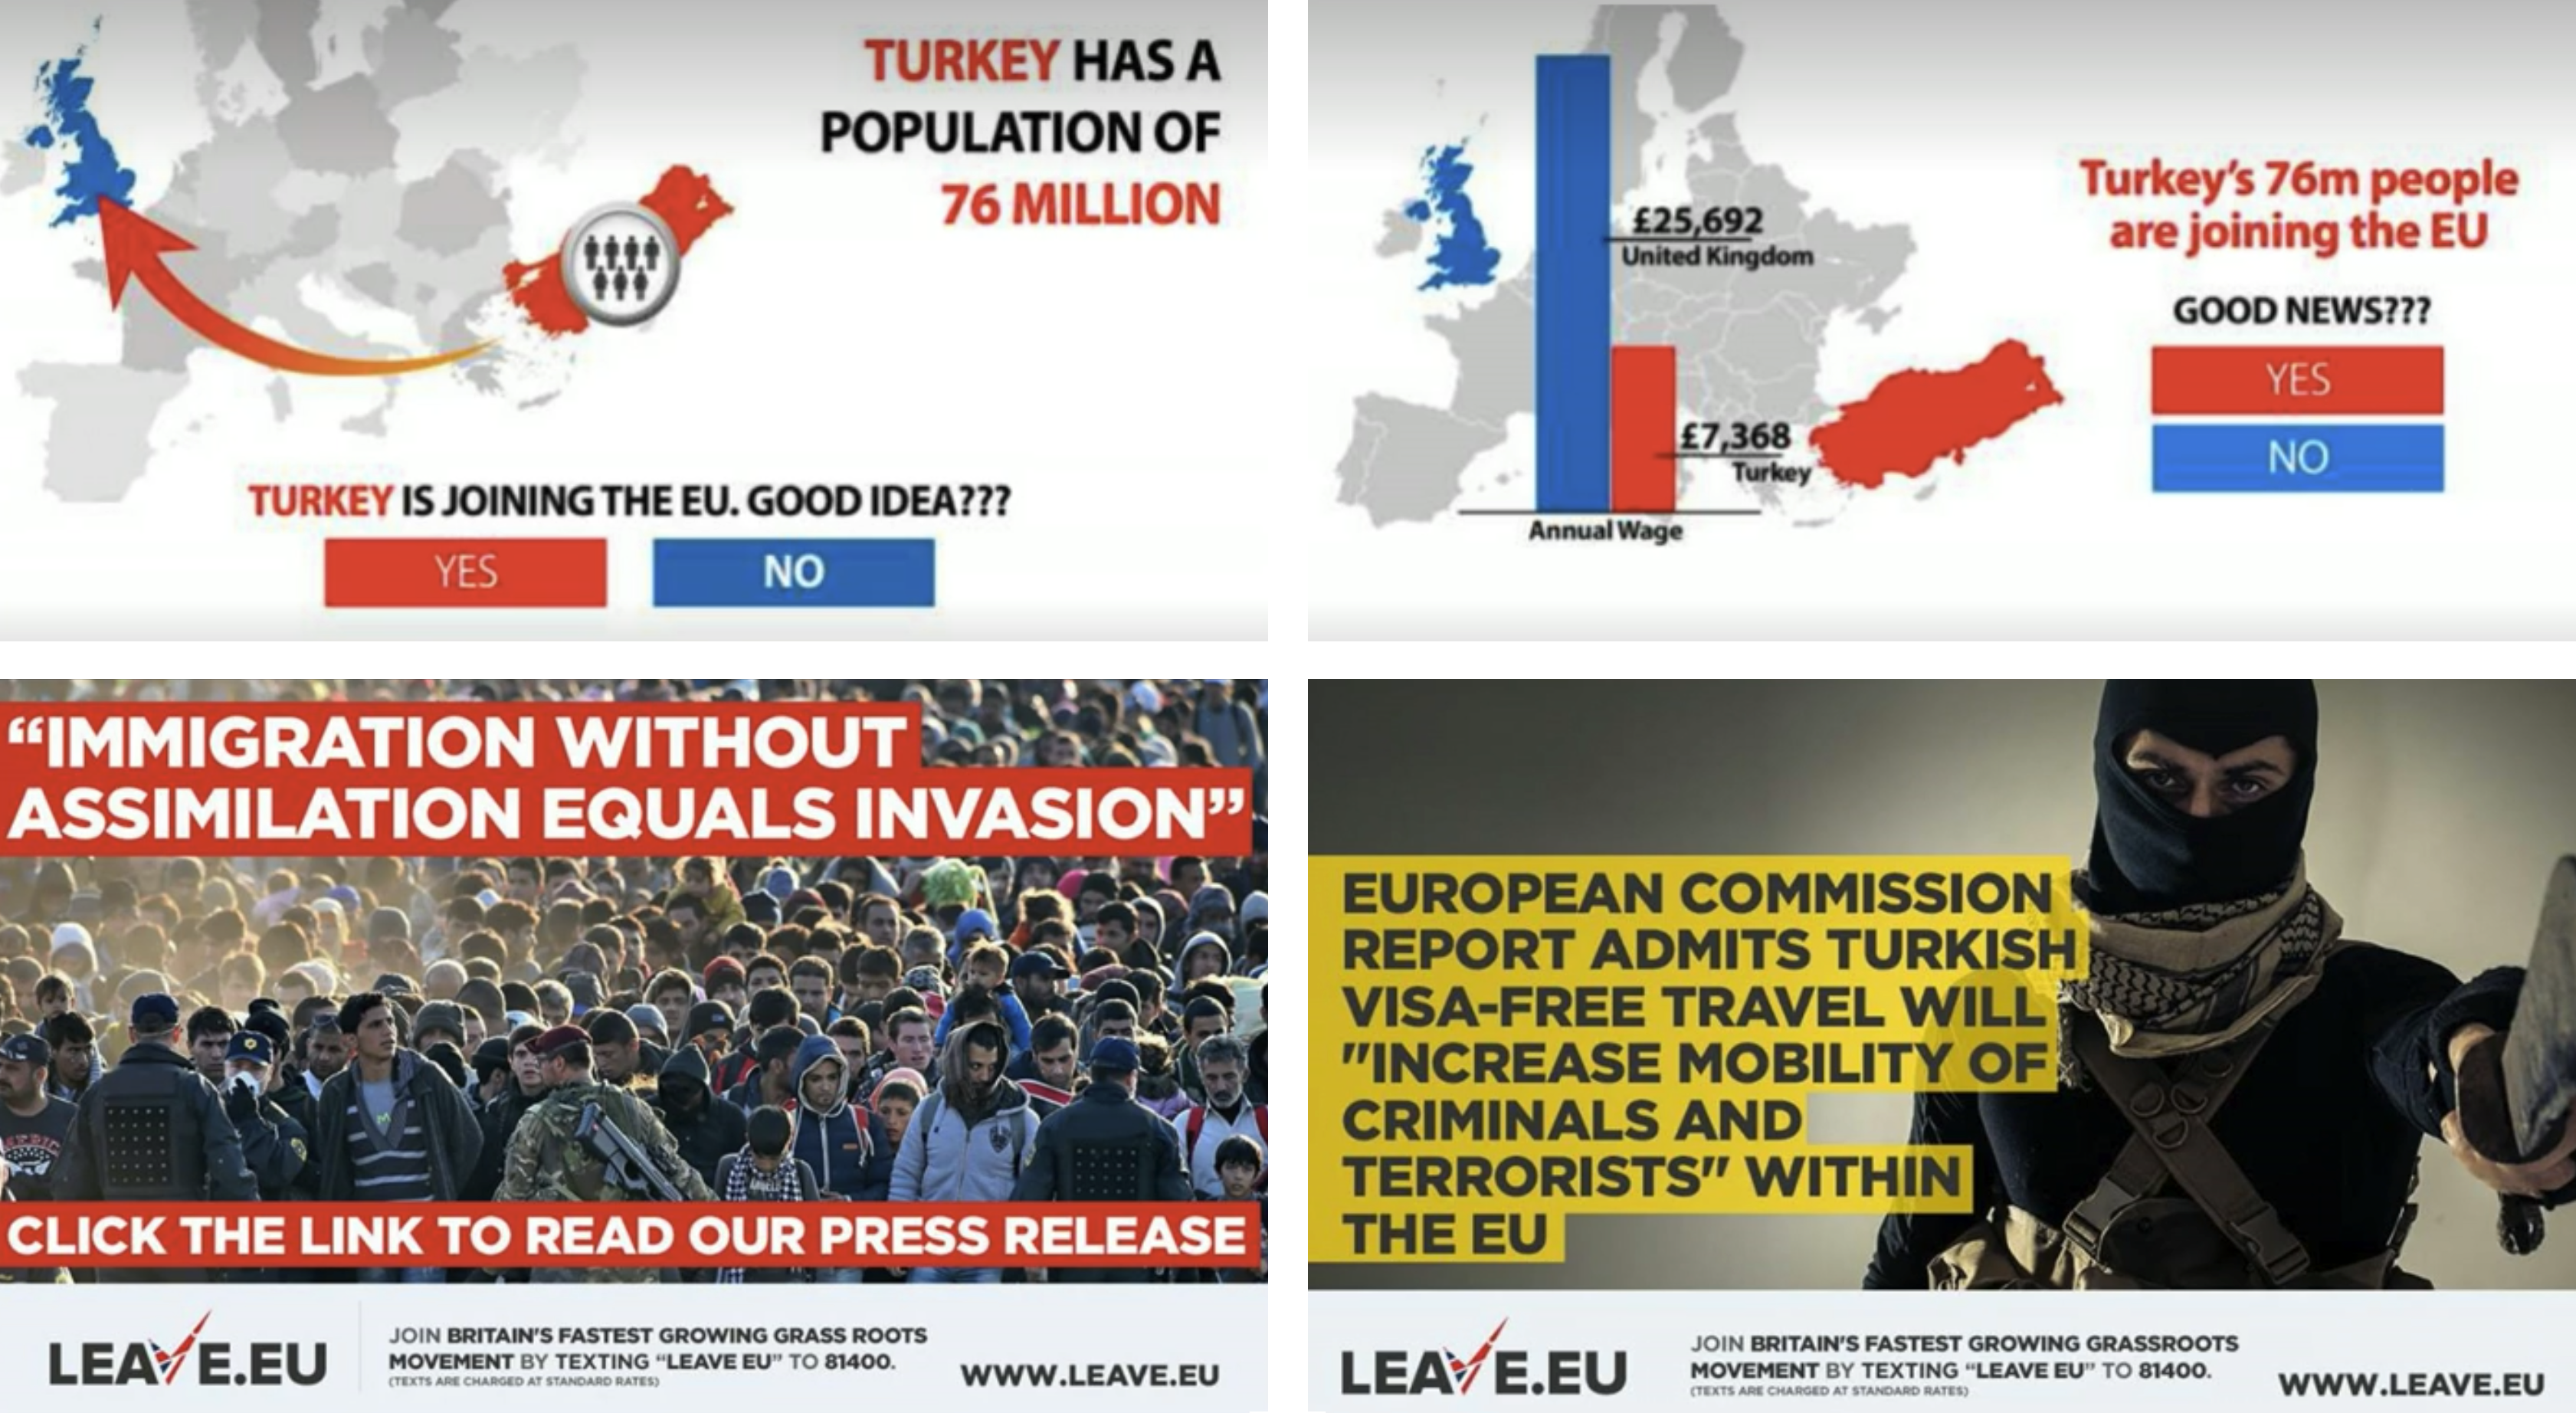
\includegraphics[width=\textwidth]{01_MotivationAndContext/figures/Fig_Brexit.png}
\caption[Targeted disinformation adverts shown on Facebook.]{Targeted disinformation adverts shown on Facebook\textsuperscript{\cite{CarCadTED}}.}
% Timestamps: 6:00, 6:10, 8:20 and 8:25 respectively.
\label{fig_Brexit}
\end{figure}

Most people in the UK saw adverts on buses and billboards with false claims that the National Health Service (NHS) would have an extra \pounds350 million a week if we left the EU. Those adverts circulated in the, open for everyone to see, making it possible to debate and debunk them in the mainstream media. The same cannot be said for the adverts in Figure \ref{fig_Brexit}. They were targeted towards specific individuals, as part of an evolving stream of information displayed in their Facebook `news' feed. The leave campaign paid Cambridge Analytica (a company that had illegally gained access to the data of 87 million Facebook users) to identify individuals that could be manipulated into voting leave. In the UK, spending on elections in the is limited by law as a means to ensure fair elections. After a nine month investigation, the UK's Electoral Commission confirmed these spending limits had been breached by the leave campaign. There are ongoing criminal investigations into where the funds for the campaign originate (overseas funding of election campaigns is also illegal) but evidence suggests ties with Russia. Brexit was the precursor to the Trump administration winning the US election just a few months later that year. The same people and companies used the same strategies. It's become clear that current legislation protecting democracy is inadequate. Facebook, was able to quietly profit from politically motivated money without recognizing any responsibility to disclose the transactions or carry out due diligence on where the money came from. Five years later, the full extent of the disinformation campaign on Facebook has yet to be understood. Who was shown what and when, how people were targeted, what other lies were told, who paid for the adverts or where the money came from.

Since then deep learning technology has advanced to the point of being able to pose as human in important ways that risk enabling disinformation not just through targeted advertising but machines impersonating humans. GANs can fabricate facial images, videos (deepfakes) and audio. Advancements in language models (Open AIs GPT-2 and more recently GPT-3) are capable of creating lengthy human like prose given just a few prompts. Deep learning now provides all the tools to fabricate human identities and target dissemination of false information at scale. There are growing concerns that in the future, bots will drown out actual human voices.

%%%%%%%%%%%%%%%%%%%%%%%%%%%%%%%%%%%%%%%%%%%%%%%%%%%%%%%%%%%%%%%%%%%%%%%%%%%%
%%%%%%%%%%%%%%%%%%%%%%%%%%%%%%%%%%%%%%%%%%%%%%%%%%%%%%%%%%%%%%%%%%%%%%%%%%%%
\subsection{Harms of allocation}

An allocative harm happens when a system allocates or withholds an opportunity or resource. Systems that approve or deny credit allocate financial resources; systems that decide who should and should not see adverts for high paying jobs allocate employment opportunities and systems that determine who will make a good tenant allocate housing resources. Harms of allocation can lead us to challenge the justice and fairness of specific determinations and outcomes. They happen as a result of discrete decisions at a given point in time, the immediate impact of which can be quantified. The methods in this book are designed to measure and mitigate harms of allocation in machine learning systems. Increasingly however, machine learning systems are not just affecting us through allocation but are shaping our view of the world and society at large by deciding what we do and don't see. Harms that are far more difficult to quantify.

%%%%%%%%%%%%%%%%%%%%%%%%%%%%%%%%%%%%%%%%%%%%%%%%%%%%%%%%%%%%%%%%%%%%%%%%%%%%
%%%%%%%%%%%%%%%%%%%%%%%%%%%%%%%%%%%%%%%%%%%%%%%%%%%%%%%%%%%%%%%%%%%%%%%%%%%%
\subsection{Harms of representation}

Harms of representation occur when systems enforce the subordination of groups through characterizations that affect the perception of them. In contrast to harms of allocation, harms of representation have long-term effects on attitudes and beliefs. They create identities and labels for humans, societies and their cultures. Harms of representation don't just affect our perception of each other, they affect how we see ourselves. They are difficult to formalise and in turn difficult to quantify but the effect is real.

\begin{lookbox}
\lbtitle{The surgeon's dilemma}
A father and his son are involved in a horrific car crash and the man died at the scene. But when the child arrived at the hospital and was rushed into the operating theatre, the surgeon pulled away and said: ``I can’t operate on this boy, he’s my son''. How can this be?
\end{lookbox}

Did you figure it out? How long did it take? There is, of course, no reason why the surgeon couldn't be the boy's mother. If it took you a while to figure out, you're not alone. More than half the people presented with this riddle struggle, and that includes women. The point of this riddle is to demonstrate the existence of unconscious bias. Representational harms are insidious. They silently fix ideas in peoples subconscious about what people of a particular gender, nationality, faith, race, occupation and more, are like. They affect our perception of world and they set boundaries for ourselves and other people. In her \href{https://www.youtube.com/watch?v=fMym_BKWQzk}{2017 NIPS keynote}, Kate Crawford described five types of harms of representation:

%%%%%%%%%%%%%%%%%%%%%%%%%%%%%%%%%%%%%%%%%%%%%%%%%%%%%%%%%%%%%%%%%%%%%%%%%%%%
\subsubsection*{Stereotyping}

Stereotyping occurs through excessively generalised portrayals of groups. In 2016 the Oxford English Dictionary was publicly criticised\cite{SexistOED} for employing the phrase ``rabid feminist'' as a usage example for the word rabid. The dictionary included similarly sexist common usages for other words like shrill, nagging and bossy. But even before this, historical linguists observed that words referring to women undergo pejoration (when the meaning of a word deteriorates over time) far more often than those referring to men\cite{Pejoration}. Examples include words such as `mistress' (once simply the female equivalent of `master' meaning a woman with authority), `hussy' (once a neutral term describing the head of a household), `madam' (once simply the female equivalent of `sir', a woman of high rank) and the list goes on.

Unsurprisingly then, gender stereotyping  is known to be a problem in natural language processing systems. In 2016 Bolukbasi et al. showed that word embeddings exhibited familiar gender biases in relation to occupations\cite{WomanHomemaker}. By performing arithmetic on word vectors, they were able to uncover relationships such as
\[
\overrightarrow{\textrm{man}} - \overrightarrow{\textrm{woman}} \approx \overrightarrow{\textrm{computer programmer}} - \overrightarrow{\textrm{homemaker}}.
\]

In 2017 Caliskan et al. found that Google Translate contained similar gender biases.\cite{BiasSemantics} In their research they found that ``translations to English from many gender-neutral languages such as Finnish, Estonian, Hungarian, Persian, and Turkish led to gender-stereotyped sentences''. So for example when they translated Turkish sentences with genderless pronouns: ``O bir doktor. O bir hemi\c{s}re.'' the resulting English sentences were: ``He is a doctor. She is a nurse.'' They performed these types of tests for 50 occupations and found that the stereotypical gender association of the word almost perfectly predicted the resulting pronoun in the English translation.

%%%%%%%%%%%%%%%%%%%%%%%%%%%%%%%%%%%%%%%%%%%%%%%%%%%%%%%%%%%%%%%%%%%%%%%%%%%%
\subsubsection*{Recognition}

Harms of recognition happen when groups of people are in some senses erased by a system through failure to recognise. In her \href{https://www.ted.com/talks/joy_buolamwini_how_i_m_fighting_bias_in_algorithms/transcript?language=en}{TED Talk}, Joy Buolamwini, talks about how as an undergraduate studying computer science she worked on social robots. One of her projects involved creating a robot which could play peek-a-boo, but she found that her robot (which used third party software for facial recognition) could not see her. She was forced to borrow her roommate's face to complete the project. After her work auditing several popular gender classification packages from IBM, Microsoft and Face++ in the project \href{http://gendershades.org/overview.html}{Gender Shades}\cite{GenderShades} in 2017 and seeing the failure of these technologies on the faces of some of the most recognizable Black women of her time, including Oprah Winfrey, Michelle Obama, and Serena Williams, she was promted to echo the words of Sojourner Truth in asking ``\href{https://medium.com/@Joy.Buolamwini/when-ai-fails-on-oprah-serena-williams-and-michelle-obama-its-time-to-face-truth-bf7c2c8a4119}{Ain't I a Woman?}''. Harms of recognition result in failures to see the humanity in people.

%%%%%%%%%%%%%%%%%%%%%%%%%%%%%%%%%%%%%%%%%%%%%%%%%%%%%%%%%%%%%%%%%%%%%%%%%%%%
\subsubsection*{Denigration}

In 2015, much to the horror of many people, it was reported that \href{https://www.bbc.com/news/technology-33347866}{Google Photos had labelled a photo of a Black couple as Gorillas}. It's hard to find the right words to describe just how offensive an error this is. It demonstrated how a machine, carrying out a seemingly benign task of labelling photos, could deliver an attack on a person's human dignity.

In 2020, an ethical audit of several large computer visions datasets\cite{TinyImages}, revealed some disturbing results. TinyImages (a dataset of 79 million 32 x 32 pixel colour photos compiled in 2006, by  MIT's Computer Science and Artificial Intelligence Lab for image recognition tasks) contained racist, misogynistic and demeaning labels with corresponding images. Figure \ref{fig_TinyImages} shows a subset of the data found in TinyImages.
%
\begin{figure}[h!]
\centering
\includegraphics[width=\textwidth]{01_MotivationAndContext/figures/Fig_TinyImages.png}
\caption[Subset of data in TinyImages exemplifying toxicity in both the images and labels.]{Subset of data in TinyImages exemplifying toxicity in both the images and labels\cite{TinyImages}.}
\label{fig_TinyImages}
\end{figure}
%
The problem, unfortunately, does not end here. Many of the datasets used to train and benchmark, not just computer vision but natural language processing tasks, are related. Tiny Images was compiled by searching the internet for images associated with words in WordNet (a machine readable, lexical database, organised by meaning, developed at Princeton), which is where TinyImages inherited its labels from. ImageNet (widely considered to be a turning point in computer vision capabilities) is also based on WordNet and, Cifar-10 and Cifar-100 were derived from TinyImages.

Vision and language datasets are enormous. The time, effort and consideration in collecting the data that forms the foundation of these technologies (compared to that which has gone into advancing the models built on them), is questionable to say the least. Furthermore a dataset can have impact beyond the applications trained on it, because datasets often don't just die, they evolve. This calls into question the technologies that are in use today, capable of creating persistent representations of our world, and trained on datasets so large they are difficult and expensive to audit.

And there's plenty of evidence to suggest that this is a problem. For example, people have found that Google searches were more likely to return personalised advertisements for arrest records searches that were suggestive of an arrest record\cite{LatanyaSweeney}. Suggestive in the sense that they claim to have arrest records specifically for the name that you searched, regardless of whether they do in reality have them. As well as resulting in allocative harms for people applying for jobs for example, this is denigrating. \href{https://www.vice.com/en_us/article/j5jmj8/google-artificial-intelligence-bias}{Google's Natural Language API for sentiment analysis also is known to have problems}. In 2017, it was assigning negative sentiment to sentences such as ``I'm a jew'' and ``I'm a homosexual'' and ``I'm black''; neutral sentiment to the phrase ``white power'' and positive sentiment to the sentences ``I'm christian'' and ``I'm sikh''.

%%%%%%%%%%%%%%%%%%%%%%%%%%%%%%%%%%%%%%%%%%%%%%%%%%%%%%%%%%%%%%%%%%%%%%%%%%%%
\subsubsection*{Under-representation}

In 2015, the New York Times reported, that ``\href{https://www.nytimes.com/2015/03/03/upshot/fewer-women-run-big-companies-than-men-named-john.html}{Fewer women run big companies than men named John}'', despite this Google's image search still managed to under-represent women in search results for the word ``CEO''. Does this really matter? What difference would an alternate set of search results make? A study the same year found that ``people rate search results higher when they are consistent with stereotypes for a career, and shifting the representation of gender in image search results can shift people’s perceptions about real-world distributions.''\cite{OccupationImageSearch}.

%%%%%%%%%%%%%%%%%%%%%%%%%%%%%%%%%%%%%%%%%%%%%%%%%%%%%%%%%%%%%%%%%%%%%%%%%%%%
\subsubsection*{Ex-nomination}

Ex-nomination occurs through invisible means and affects people's views of the norms within societies. It tends to happen through mechanisms which amplify the presence of some groups and suppress the presence of others. The cultures, beliefs, politics of ex-nominated groups over time become the default. The most obvious example is the ex-nomination of Whiteness and White culture in western society, which might sound like a bizarre statement - what is White culture? But such is the effect of ex-nomination, you can't describe it, because it is just the norm and everything else is not. Richard Dyer in his book White examines the reproduction and preservation of whiteness in visual media over five centuries, from the depiction of the crucifixion to modern day film. It's should hardly come as a surprise then that facial recognition software might not see black faces and more often incorrectly identify the gender of black women. Or that an image of generative model called Pulse converted a pixelated picture of Barack Obama, into a high-resolution image of a white man.

The ex-nomination of White culture is evident in our language too, in terminology like whitelist and white lie. If you look up white in dictionary and or thesaurus and you'll find words like innocent and pure, light, transparent, immaculate, neutral. Doing the same for the word black on the other hand, returns very different associations, dirty, soiled, evil, wicked, black magic, black arts, black mark, black humour, blacklist and black is often used as a prefix in describing disastrous events. A similar assessment can be made for gender with women being under-represented in image data and feminine versions of words more often undergoing pejoration (when the meaning or status of a word deteriorates over time). Consider the words mistress (once simply the female equivalent of master, now used to describe a woman in a relationship with a man married to another); madam (once simply the female equivalent of sir, now also used to describe a woman who runs a brothel); hussy (once a neutral term for the head of a household, now used to describe a woman who has sexual relationships with multiple partners); and governess (female equivalent of governor, later used to describe a woman responsible for the care of children).

Members of ex-nominated groups experience a kind of privilege that it is easy to be unaware of. It is a power that comes from being the norm. They have advantages that are not earned, outside of their financial standing or effort, that the `equivalent' person outside the ex-nominated group would not. Their hair type, skin tone, accent, food preferences and more are catered to by every store, product, service and system and it cost less to access them; they see themselves represented in the media and are more often represented in a positive light; they are not subject to profiling or stereotypes; they are more likely to be treated as individuals rather than as representative of (or as exceptions to) a group; they are more often humanised - more likely to be be given the benefit of the doubt, treated with compassion and kindness and thus recover from mistakes; they are less likely to be suspected of crimes; more likely to be trusted financially; they have greater access to opportunities, resources and power and are able to climb financial, social and professional ladders faster. The advantages enjoyed by ex-nominated groups accumulate over time and compound over generations.

%%%%%%%%%%%%%%%%%%%%%%%%%%%%%%%%%%%%%%%%%%%%%%%%%%%%%%%%%%%%%%%%%%%%%%%%%%%%
%%%%%%%%%%%%%%%%%%%%%%%%%%%%%%%%%%%%%%%%%%%%%%%%%%%%%%%%%%%%%%%%%%%%%%%%%%%%
%%%%%%%%%%%%%%%%%%%%%%%%%%%%%%%%%%%%%%%%%%%%%%%%%%%%%%%%%%%%%%%%%%%%%%%%%%%%
\section*{Summary}
\addcontentsline{toc}{section}{Summary}

%%%%%%%%%%%%%%%%%%%%%%%%%%%%%%%%%%%%%%%%%%%%%%%%%%%%%%%%%%%%%%%%%%%%%%%%%%%%
%%%%%%%%%%%%%%%%%%%%%%%%%%%%%%%%%%%%%%%%%%%%%%%%%%%%%%%%%%%%%%%%%%%%%%%%%%%%
\subsection*{Machine learning}

\begin{itemize}[leftmargin=*]
\item A model is a simplified representation of the real world. Machine learning models are trained on historic data and best capture the dense part of the distribution. When faced with rare or unprecedented events they will struggle to perform well. Obtaining adequately rich and relevant data is a major limitation for most machine learning models.
%
\item At almost every major life event, going to university, getting a job, buying a house, getting sick, decisions are increasingly being made by machines. By construction, these models encode existing societal biases. They not only proliferate but are capable of amplifying them and are easily deployed at scale. Understanding the shortcomings of these models and ensuring such technologies are deployed responsibly are essential if we are to safeguard social progress.
\end{itemize}

%%%%%%%%%%%%%%%%%%%%%%%%%%%%%%%%%%%%%%%%%%%%%%%%%%%%%%%%%%%%%%%%%%%%%%%%%%%%
%%%%%%%%%%%%%%%%%%%%%%%%%%%%%%%%%%%%%%%%%%%%%%%%%%%%%%%%%%%%%%%%%%%%%%%%%%%%
\subsection*{Discrimination, bias, fairness and ethics}

\begin{itemize}[leftmargin=*]
\item Building machine learning systems ethically is not about finding the perfect answer every time but rather expanding our perspectives on the technology we develop. It’s looking for the cracks before deploying systems, preventing the foreseeable failures and doing the best we can on the ones we didn’t see coming.
%
\item The standard, approach to training a model, which is essentially to minimise the aggregate error on the training data, is loosely justified in a utilitarian sense, in that we choose the decision process which maximises accuracy (minimises the probability of error) for the greatest number of people (everyone in the training data).
%
\item Principles of Justice as Fairness:
%
\begin{enumerate}[leftmargin=*]
\item \textbf{Liberty principle:} Each person has the same indefeasible claim to a fully adequate scheme of equal basic liberties, which is compatible with the same scheme of liberties for all;
\item \textbf{Equality principle:} Social and economic inequalities are to satisfy two conditions:
\begin{enumerate}[leftmargin=*]
\item \textbf{Fair equality of opportunity:} The offices and positions to which they are attached are open to all under conditions of fair equality of opportunity;
\item \textbf{Difference principle} They must be of the greatest benefit to the least-advantaged members of society.
\end{enumerate}
\end{enumerate}
%
The principles of justice as fairness are ordered by priority so that fulfilment of the liberty principle takes precedence over the equality principles and fair equality of opportunity takes precedence over the difference principle. In contrast to utilitarianism, justice as fairness introduces a number of constraints that must be satisfied for a decision process to be fair. Applied to a machine learning one might interpret the liberty principle as a requirement of some minimum accuracy level (maximum probability of error) to be set for all members of the population, even if this means the algorithm is less accurate overall. Parallels can be drawn here in machine learning where there is a trade-off between fairness and utility of an algorithm.
%
\item Anti-discrimination laws were born out of long-standing, vast and systemic discrimination against historically oppressed and disadvantaged classes. Such discrimination has contributed to disparities in all measures of prosperity (health, wealth, housing, crime, incarceration) that persist today.
%
\item Legal liability for discrimination against protected classes may be established through both disparate treatment and disparate impact. Disparate treatment (also described as direct discrimination in Europe) refers to both formal differences in the treatment of individuals based on protected characteristics, and the intent to discriminate. Disparate impact (also described as indirect discrimination in Europe) does not consider intent but is concerned with policies and practices that disproportionately impact protected classes.
%
\item Just as the meaning of fairness is subjective, so too is the interpretation of anti-discrimination laws. Two conflicting interpretations are anti-classification and anti-subordination. Anti-classification is a weaker interpretation, that the law is intended to prevent classification of people based on protected characteristics. Anti-subordination is the stronger interpretation that anti-discrimination laws exist to prevent social hierarchies, class or caste systems based on protected features and, that it should actively work to eliminate them where they exist.
\end{itemize}

%%%%%%%%%%%%%%%%%%%%%%%%%%%%%%%%%%%%%%%%%%%%%%%%%%%%%%%%%%%%%%%%%%%%%%%%%%%%
%%%%%%%%%%%%%%%%%%%%%%%%%%%%%%%%%%%%%%%%%%%%%%%%%%%%%%%%%%%%%%%%%%%%%%%%%%%%
\subsection*{Association paradoxes}

\begin{itemize}[leftmargin=*]
\item Identifying bias in data can be tricky. Data can be misleading. An association paradox is a phenomenon where an observable relationship between two variables disappears or reverses after controlling for one or more other variables. In such cases in order to know if the marginal or partial relationships are relevant, one must understand the causal nature of the relationships. Association paradoxes can also occur for non-collapsible measures of association. Collapsible measures of association are those which can be expressed as the weighted average of the partial measures.
\end{itemize}

%%%%%%%%%%%%%%%%%%%%%%%%%%%%%%%%%%%%%%%%%%%%%%%%%%%%%%%%%%%%%%%%%%%%%%%%%%%%
%%%%%%%%%%%%%%%%%%%%%%%%%%%%%%%%%%%%%%%%%%%%%%%%%%%%%%%%%%%%%%%%%%%%%%%%%%%%
\subsection*{Harms of unfair bias}

\begin{itemize}[leftmargin=*]
\item It is important to be cautious in describing machine learning algorithms as objective. Algorithms trained on data are exposed to bias since data is produced by a necessarily subjective set of decisions. The consistency of algorithms in decision making compared to humans (who make decisions on a case by case basis) is often described as a benefit, but it's their very consistency that makes them dangerous - capable of discriminating systematically and at scale.
%
\item Classification creates a sense of order and understanding. It enables us to formulate problems neatly and solve them. But classifying people can also have negative consequences too. It inevitably has the effect of reducing people labels; labels that can result in people being treated as members of a group, rather than individuals.
%
\item Personalisation algorithms that shape our perception of the world in a way that covertly mirror our beliefs can have the effect of decreasing bridging capital which is important in solving global problems.
%
\item Targeted political advertising and technologies that enable machines to impersonate humans are powerful tools that can be used as part of orchestrated campaigns of disinformation that manipulate perceptions at an individual level and yet at scale. They are capable of causing great harm to political and social institutions and pose a threat to security. 
%
\item An allocative harm happens when a system allocates or withholds an opportunity or resource. Harms of representation occur when systems enforce the subordination of groups through characterizations that affect the perception of them. In contrast to harms of allocation, harms of representation have long-term effects on attitudes and beliefs. They create identities and labels for humans, societies and their cultures. Harms of representation affect our perception of each other and even ourselves. Harms of representation are difficult to quantify. Some types of harms of representation are, stereotyping, (failure of) recognition, denigration, under-representation and ex-nomination.
\end{itemize}

%%%%%%%%%%%%%%%%%%%%%%%%%%%%%%%%%%%%%%%%%%%%%%%%%%%%%%%%%%%%%%%%%%%%%%%%%%%%
\bibliographystyle{plain}
\bibliography{99_BackMatter/References}
